\chapter{Detector description}

%versions of the detector
\section{History}

``The desktop muon detector was initially built as a Muon Tagging Optical Modules (MTOMs) for PINGU, the proposed low energy upgrade for IceCube experiment'' \cite{CosmicWatch}. Since the first iteration, CosmicWatch has had multiple versions, always aiming to reduce size and costs, simplify its construction, and provide better documentation for new CosmicWatch users. An in-depth review of the detector evolution can be found in \cite{CosmicWatch} under ``About the project/Project evolution''.

The prototypes of CosmicWatch Fig. \ref{sfig:CW_ver1} used liquid scintillator, this however proved to be inefficient, since it was prone to leaks. The second prototype used a $5\times5\times5$ \unit{\cm\cubed} plastic scintillator in a light-tight reflective aluminum case Fig. \ref{sfig:CW_ver2}, this was however too slow, large, and expensive, making it not suitable for students.

\begin{figure}[H]
  \centering
  \begin{subfigure}[t]{0.45\textwidth}
    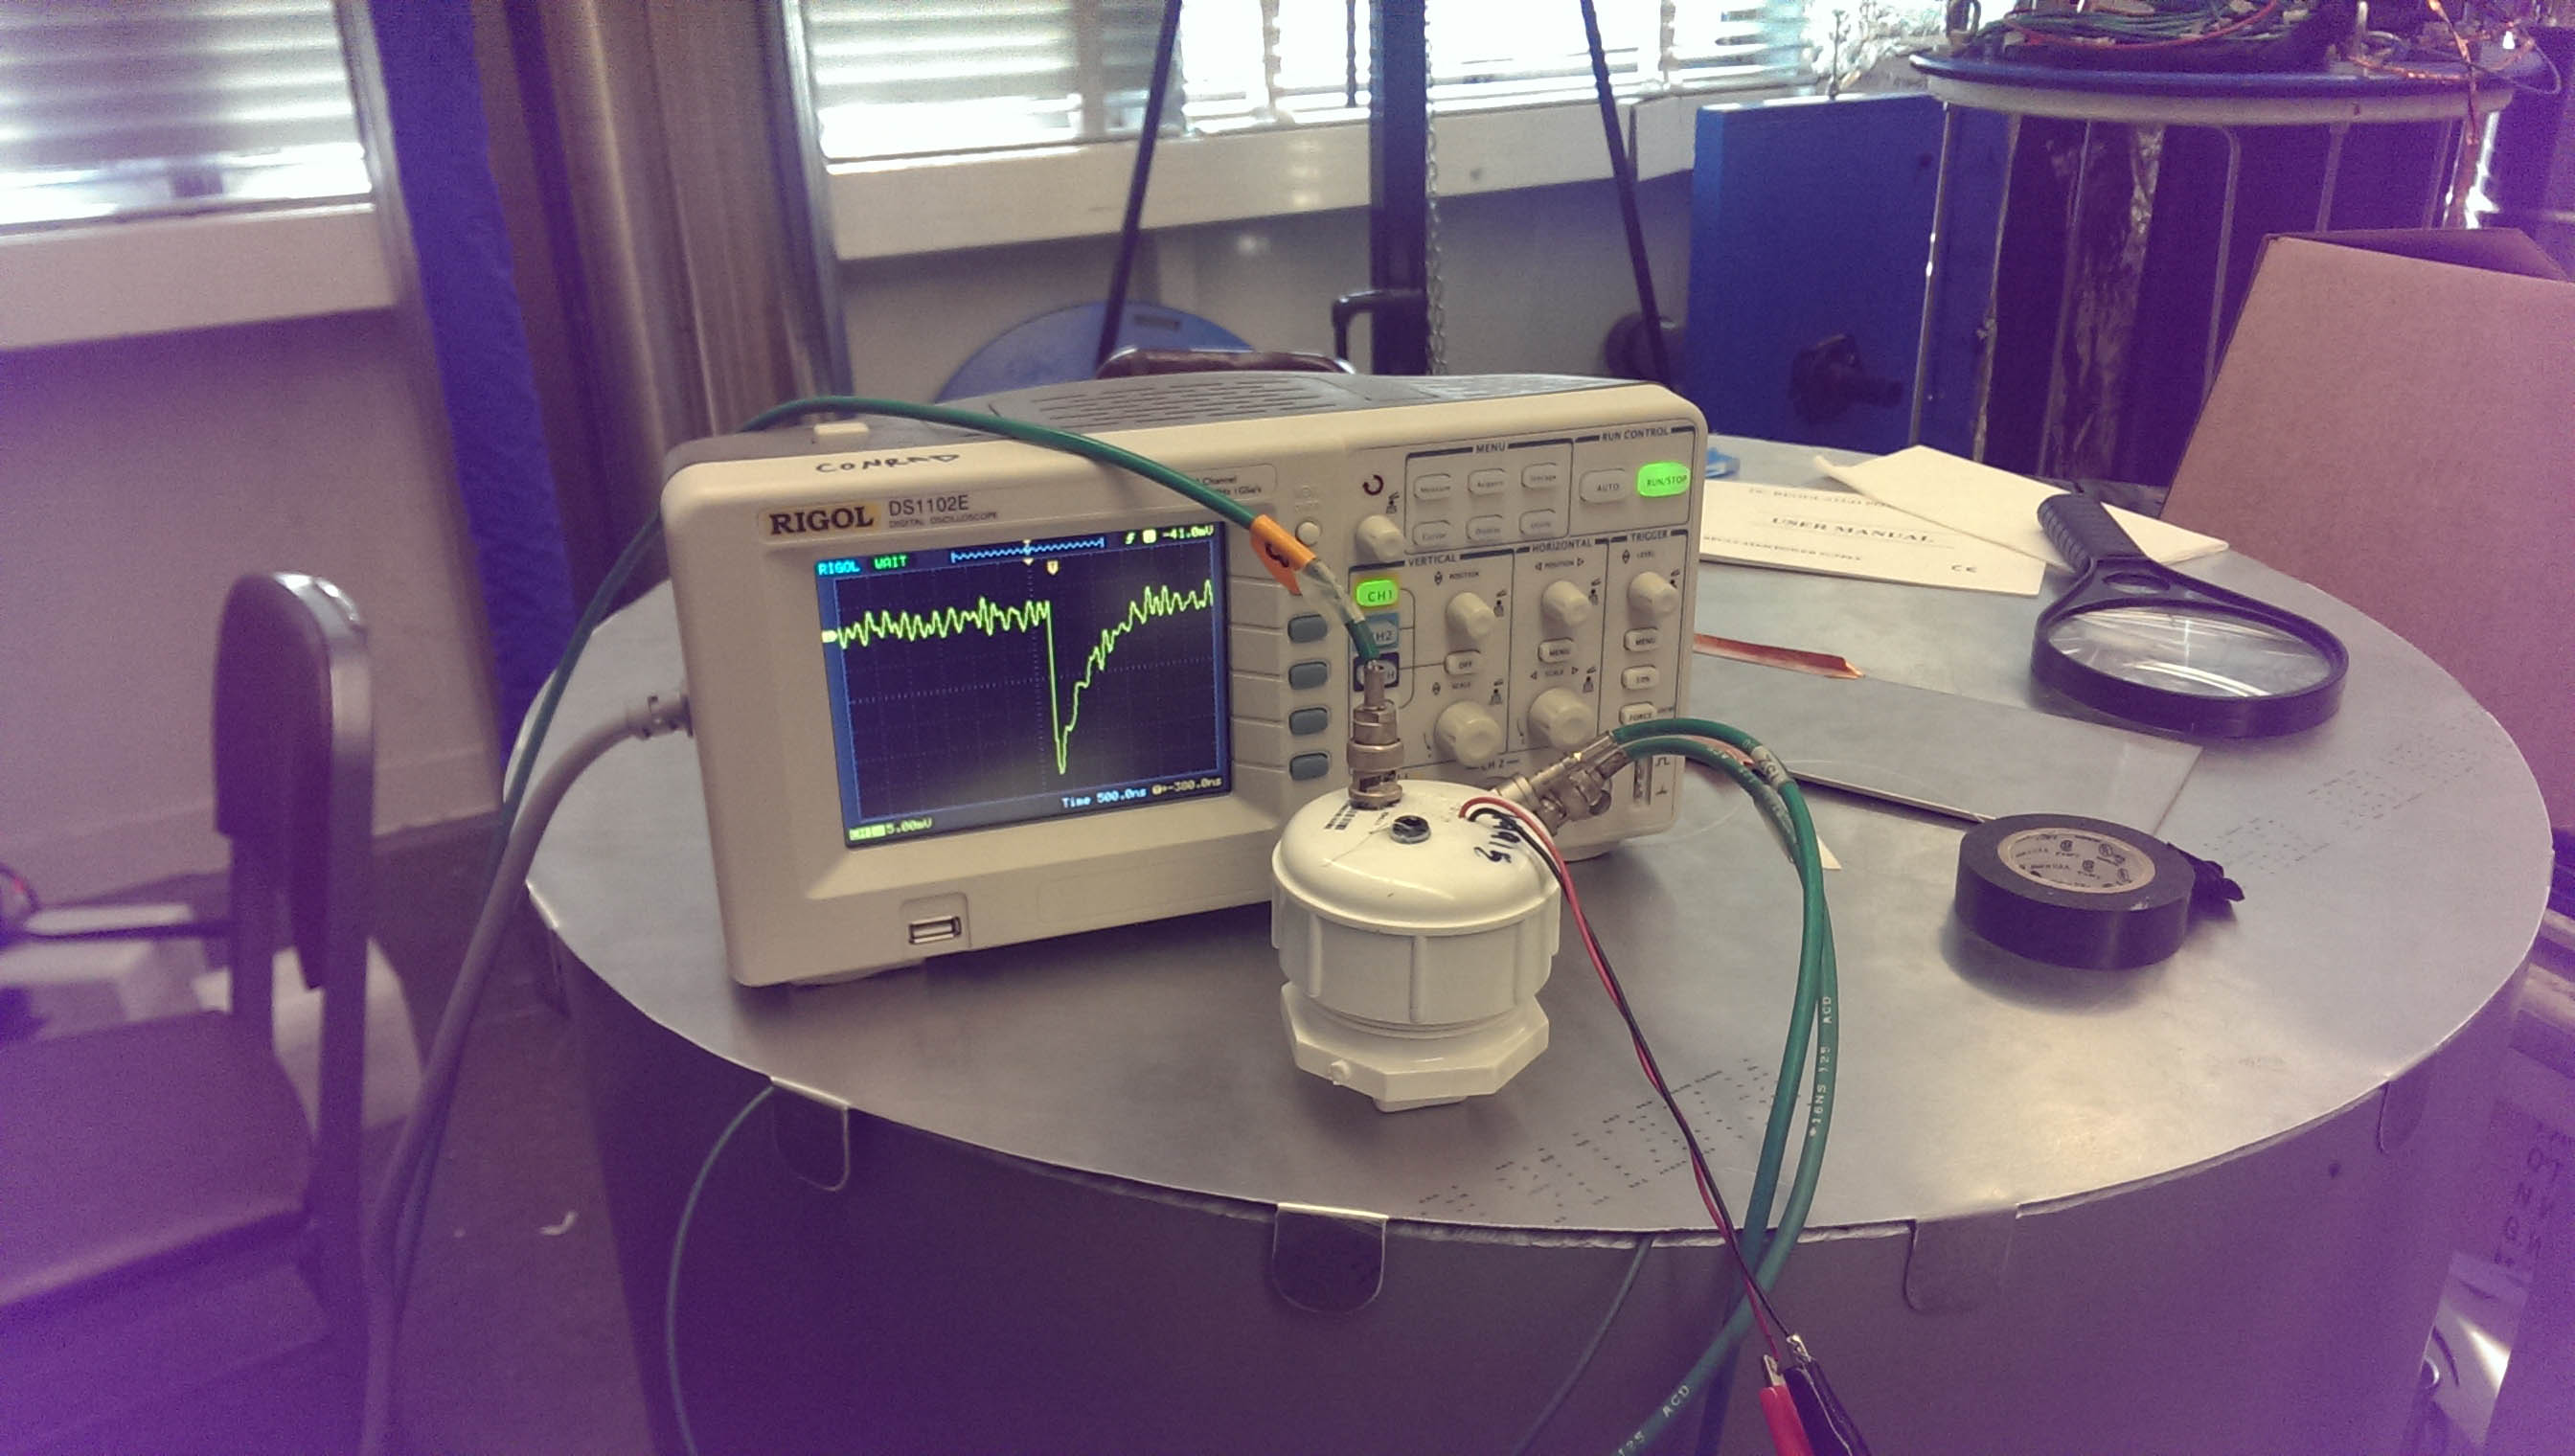
\includegraphics[width=\textwidth]{Detector_description/CW-ver1.jpg}
    \caption{\label{sfig:CW_ver1} First prototype}
  \end{subfigure}
  \begin{subfigure}[t]{0.45\textwidth}
    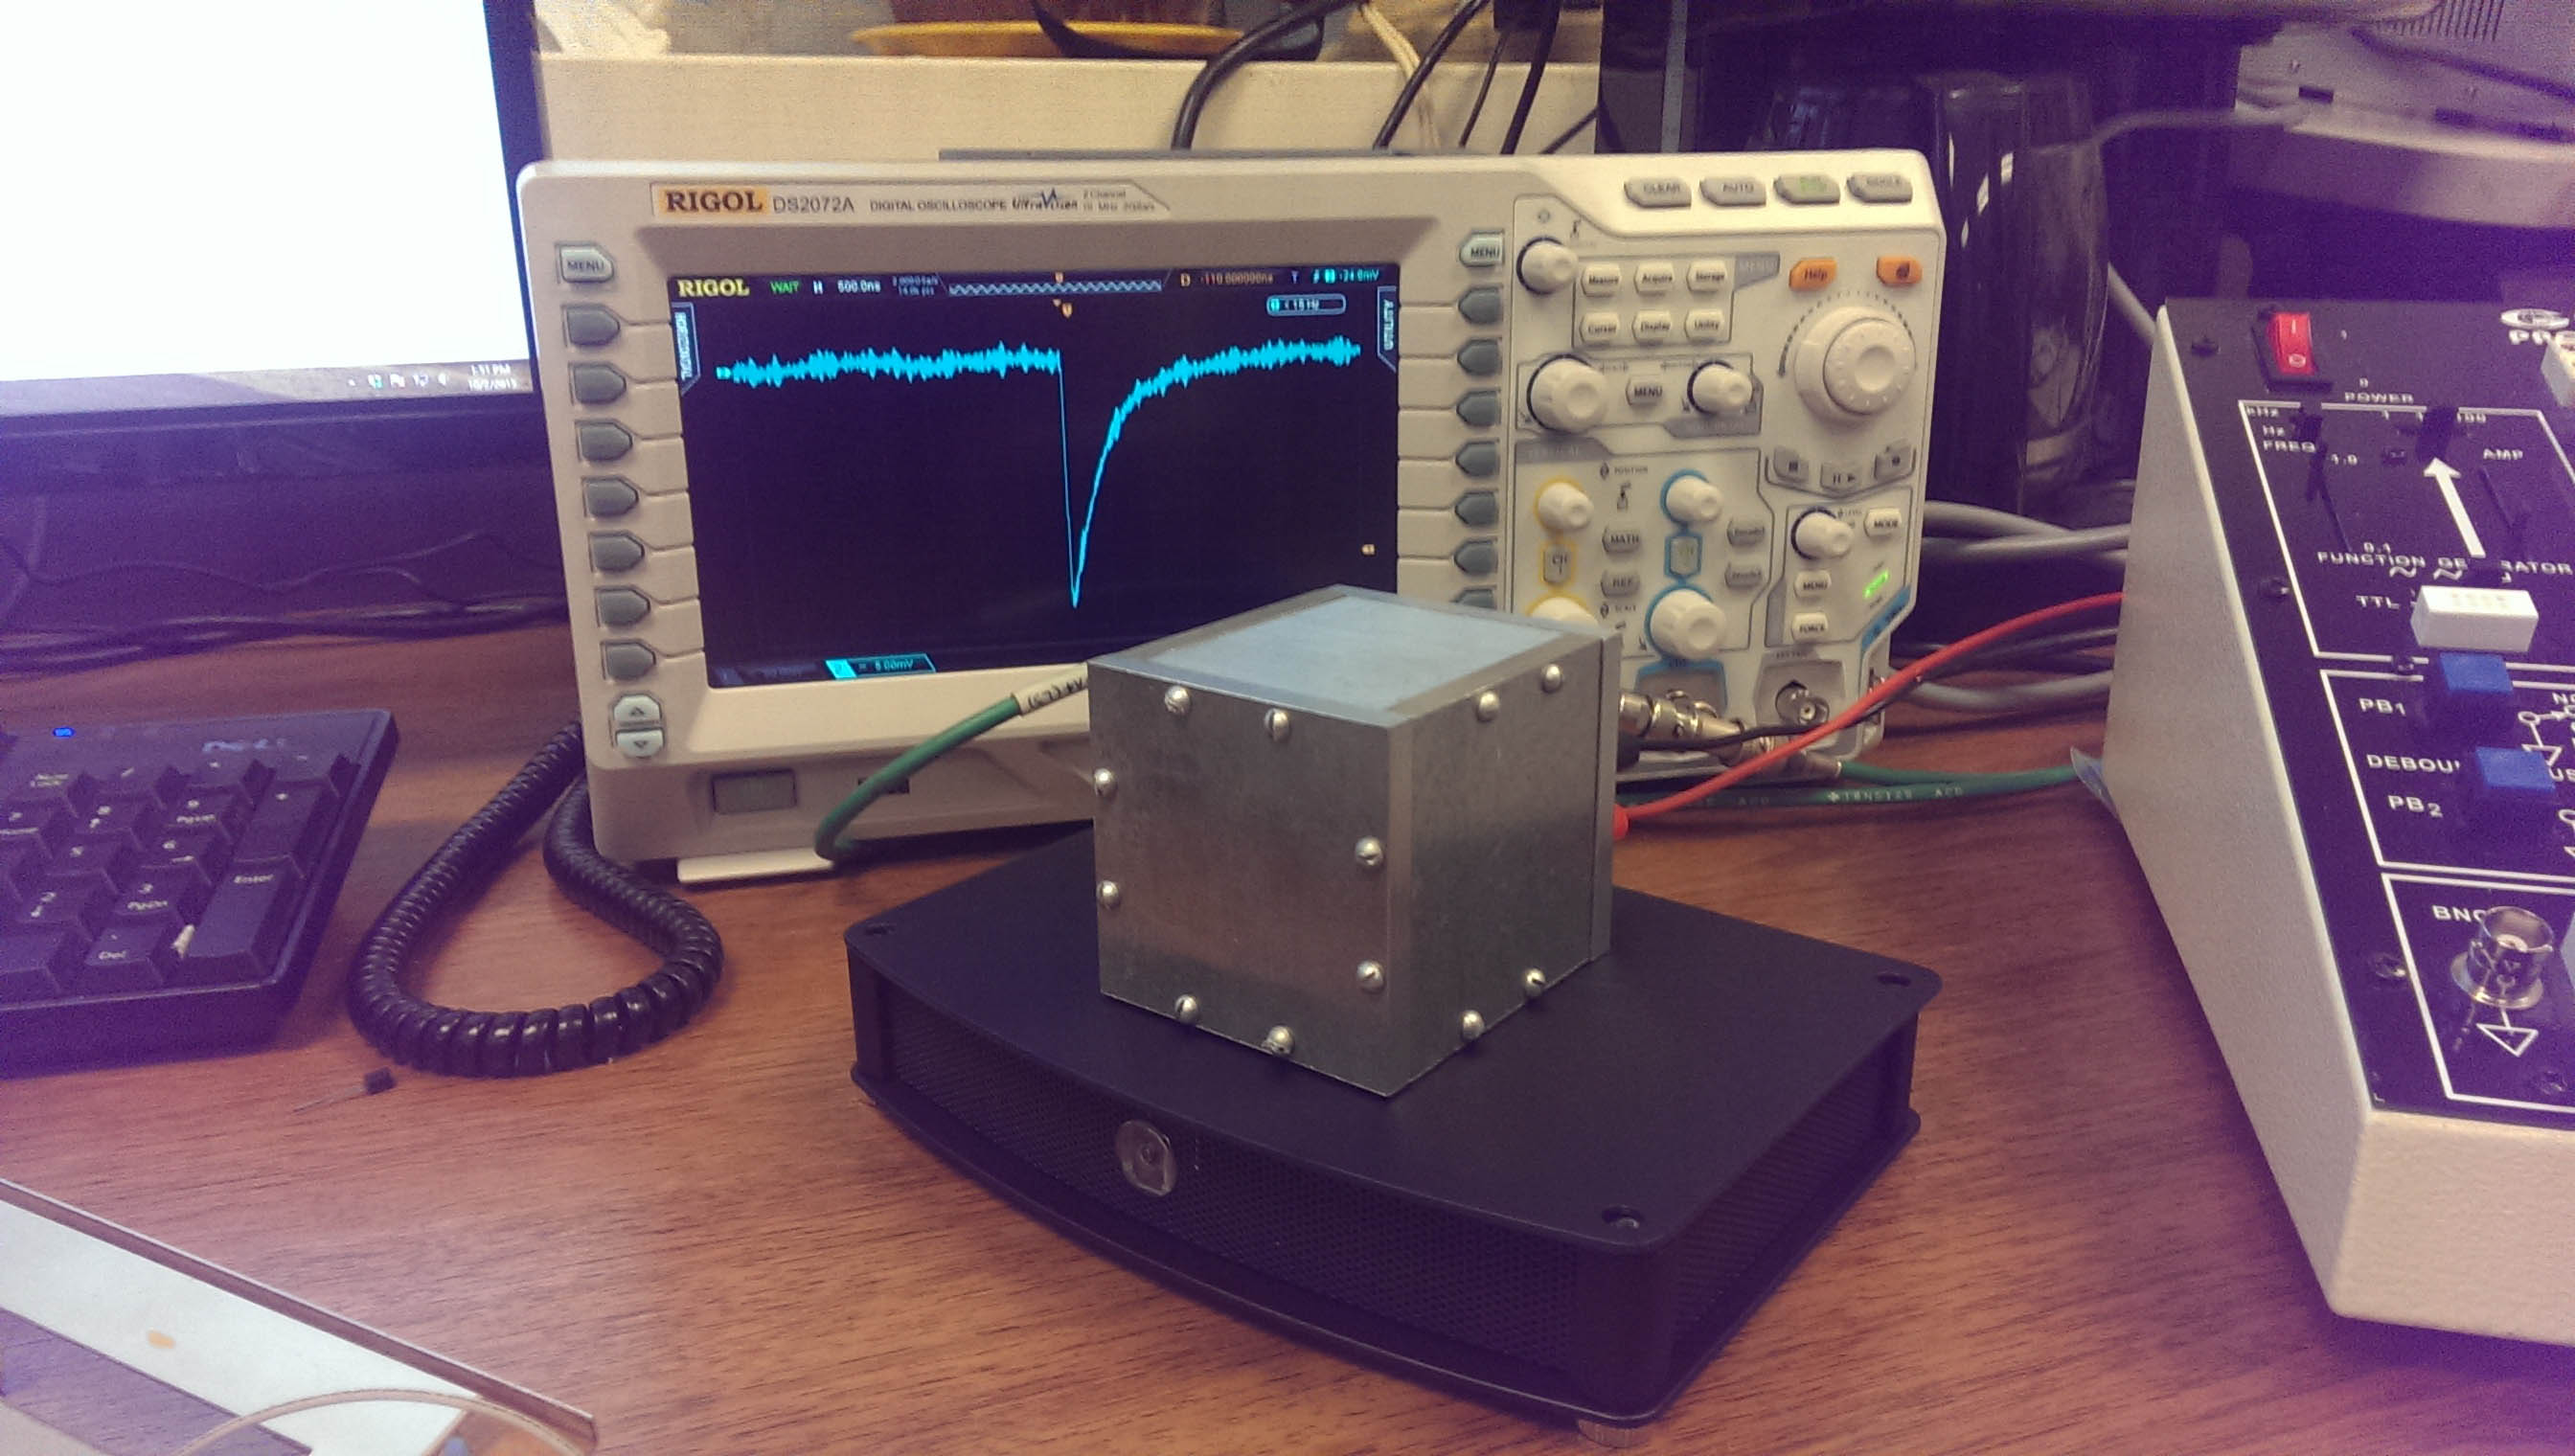
\includegraphics[width=\textwidth]{Detector_description/CW-ver2.jpg}
    \caption{\label{sfig:CW_ver2} Second prototype}
  \end{subfigure}
  \caption{\label{fig:CW_ver1_ver2}First versions of CosmicWatch, prototypes for PINGU, taken from \cite{CosmicWatch}.}
\end{figure}

Later iterations resemble the current goals of CosmicWatch, they are cheaper, smaller, and easier to build. Versions 1 and 2 (Fig. \ref{sfig:CW_ver3}) introduced some user-friendly features, including battery/USB power with $~0.3$ \unit{\watt} consumption, a software-adjustable trigger threshold, and cost about \$100. V2 in particular introduced the use of SD cards to save data and the capability to connect two CosmicWatches, making it possible to measure coincident events.

\begin{figure}[H]
  \centering
  \begin{subfigure}[t]{0.45\textwidth}
    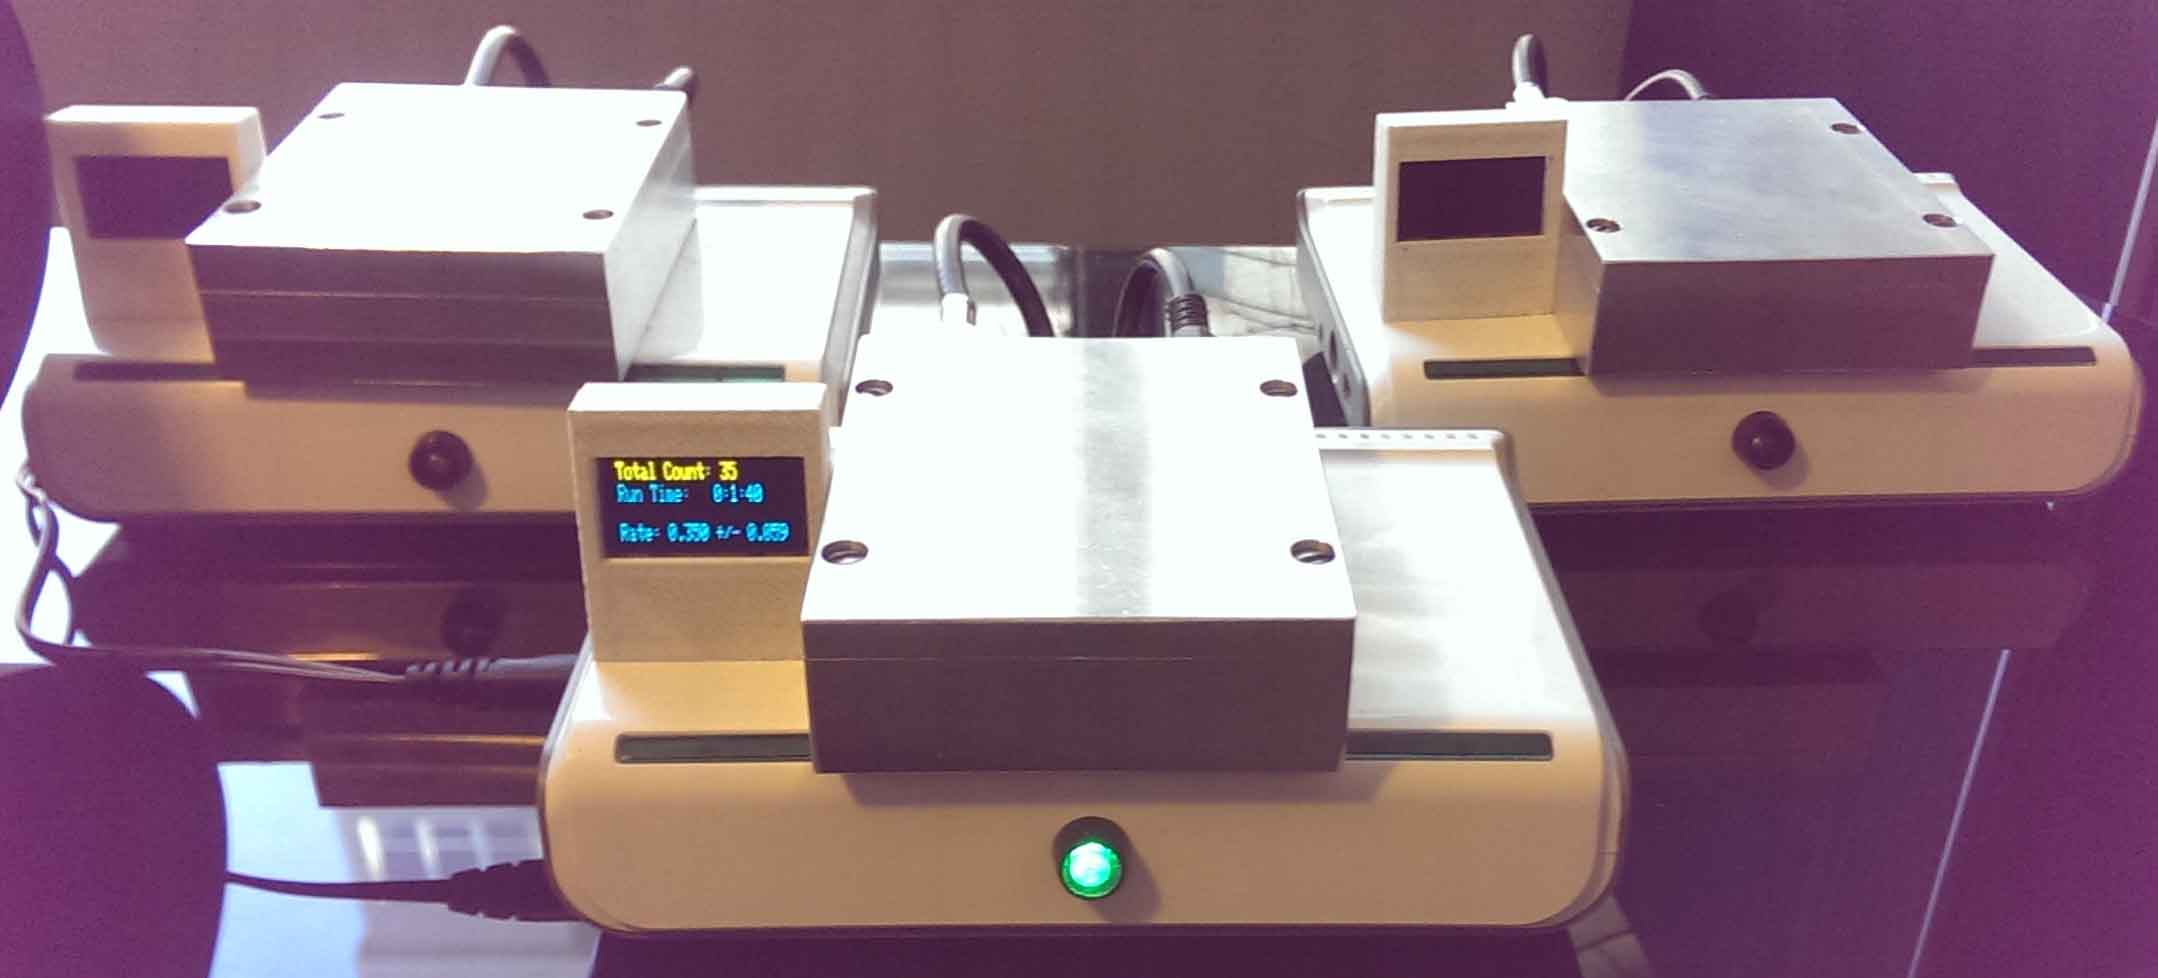
\includegraphics[width=\textwidth]{Detector_description/CW-ver3.jpg}
    \caption{\label{sfig:CW_ver3} Third prototype}
  \end{subfigure}
  \begin{subfigure}[t]{0.45\textwidth}
    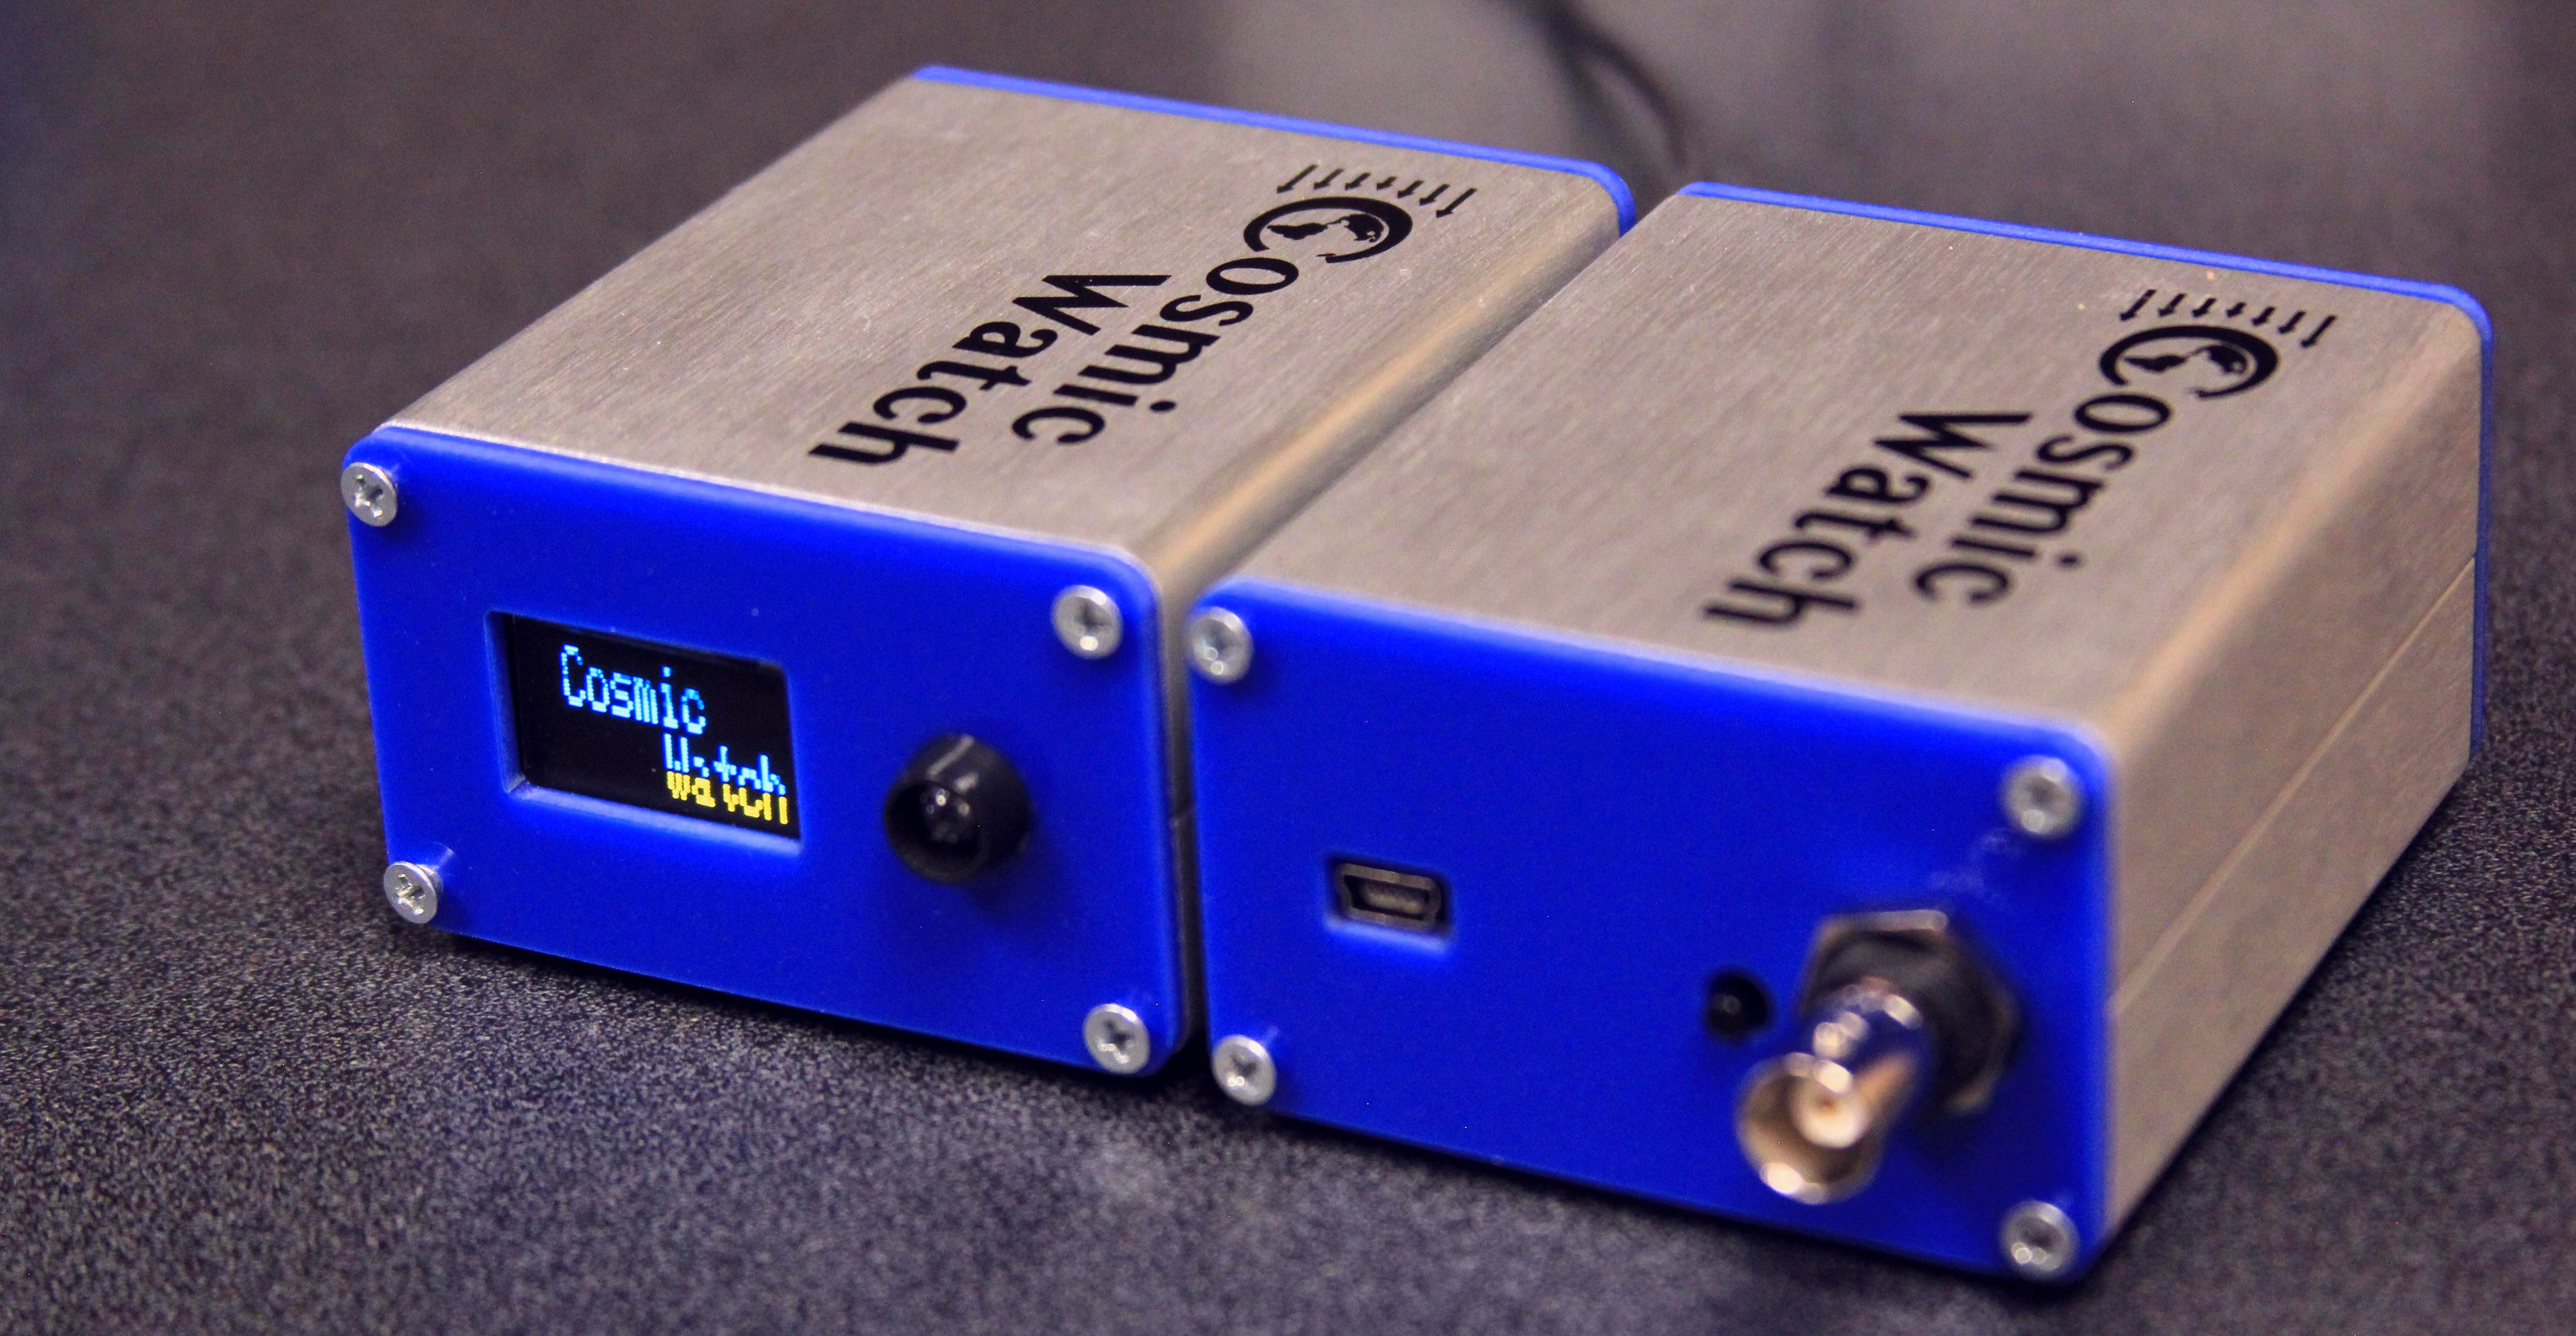
\includegraphics[width=\textwidth]{Detector_description/CW_ver4.jpeg}
    \caption{\label{sfig:CW_ver4} CosmicWatch versions 1 and 2}
  \end{subfigure}
  \caption{\label{fig:CW_ver3_ver4}Newer versions of CosmicWatch, designs suitable for students, taken from \cite{CosmicWatch}.}
\end{figure}

The previous versions of CosmicWatch used an Arduino Nano to process the signal coming from the photomultiplier\footnote{See chapter \ref{chap:Electronics} for an in-depth description of the inner workings of the detector electronics}, which has only one core. This is a disadvantage when there is a high event rate since one can not sample data while saving previous events. The use of a Raspberry Pi Pico is one of the main improvements in upcoming versions of CosmicWatch, its two cores allow to sample data in one thread while the other handles serial communication to save previous events. This will reduce deadtime, making it suitable for high event rates, such as those found around active gamma sources.

\section{Plastic vs. LYSO}

Up until now, due to how affordable and malleable they can be, only plastic scintillators have been used, particularly Polyvinyltoluene-based scintillators such as BC-400 and BC404. Sadly, it is well known that their poor energy resolution and lack of linearity makes them useless for gamma spectroscopy, at least in small sizes as the ones used for CosmicWatch ($5\times5\times1$ \unit{\cm\cubed}). In addition to this, plastic scintillators have very low light yields $10000$ photons/MeV \cite{mukhopadhyay2004plastic}, making it hard to detect low-energy events. Table \ref{tab:scintillators} compares the general properties of some scintillating materials, better showcasing the advantages of LYSO in particular for gamma spectroscopy in the CosmicWatch context.

\begin{table}[htb]
  \caption{General properties of some scintillating materials. Taken from \cite{mukhopadhyay2004plastic,Luxium_LYSO,Luxium_plastic,SaintGobain_NaI}. $^*$Calculated from the attenuation coefficient at 662 \unit{\kilo\eV} shown in \cite[p.~3]{SaintGobain_NaI}}
  \centering
  \begin{tabular}{ l c c c c}
    \midrule
    Property & LYSO & BC-400 & NaI(TI) & BGO\\
    \midrule
    Density [\unit{\g\per\cm\cubed}] & 7.1 & 1.032 & 3.67 & 7.1\\
    Decay time [\unit{\nano\s}]  & 36 & 2.4 & 250 & 300\\
    Light yield [\unit{ph\per\mega\eV}] & 33200 & 10000 & 38000 & 9000\\
    Attenuation Length at 511 \unit{\kilo\eV} [\unit{\cm}] & 1.2 &  & $3.3^{*}$ & 1.0\\
    \bottomrule
  \end{tabular}
  \label{tab:scintillators}
\end{table}

Higher densities are good for energy deposition, catching particles and gammas more efficiently. Short decay times allow to make fast signal pulses. High light yields make it possible to detect low-energy events. Short attenuation lengths decrease the amount of material necessary to get energy depositions.

\section{Power Consumption}

\section{KiCad}

KiCad is an open-source software that allows the creation of circuit schematics, PCB layout, and 3D viewing among other capabilities. It is available in Windows, Linux, and iOS, making it perfect for CosmicWatch, since one of the goals is to make it easily available to new users. The KiCad project for CosmicWatch V2 can be found on the repository \href{https://github.com/spenceraxani/CosmicWatch-Desktop-Muon-Detector-v2}{CosmicWatch-Desktop-Muon-Detector-v2} under ``PCB\_Files''.

\href{https://github.com/anvargasl/CosmicWatch-gamma-spectroscopy-PCB}{CosmicWatch-gamma-spectroscopy-PCB} contains the KiCad files necessary to build the newer version of CosmicWatch, all the necessary footprints can be found in ``MyLibrary.pretty'', including the Raspberry Pi Pico footprints. In order to print the PCB, it is necessary to send the compressed ``Geber'' folder (found under ``CosmicWatch\_detector\_v33'') to a manufacturer, \href{https://www.elecrow.com/pcb-manufacturing.html}{ELECROW} is recommended.

\section{Accessories}

Currently, CosmicWatch includes some accessories that make it possible to customize the detector and get more specific measurements, making use of its multiple sensors and features. Drivers and example code necessary to control the accessories listed below are included in \href{https://github.com/anvargasl/CosmicWatch-gamma-spectroscopy-RP}{CosmicWatch-gamma-spectroscopy-RP} under the ``drivers'' folder.

\subsection{Preassure and Temperature sensor}

\begin{figure}[H]
  \centering
  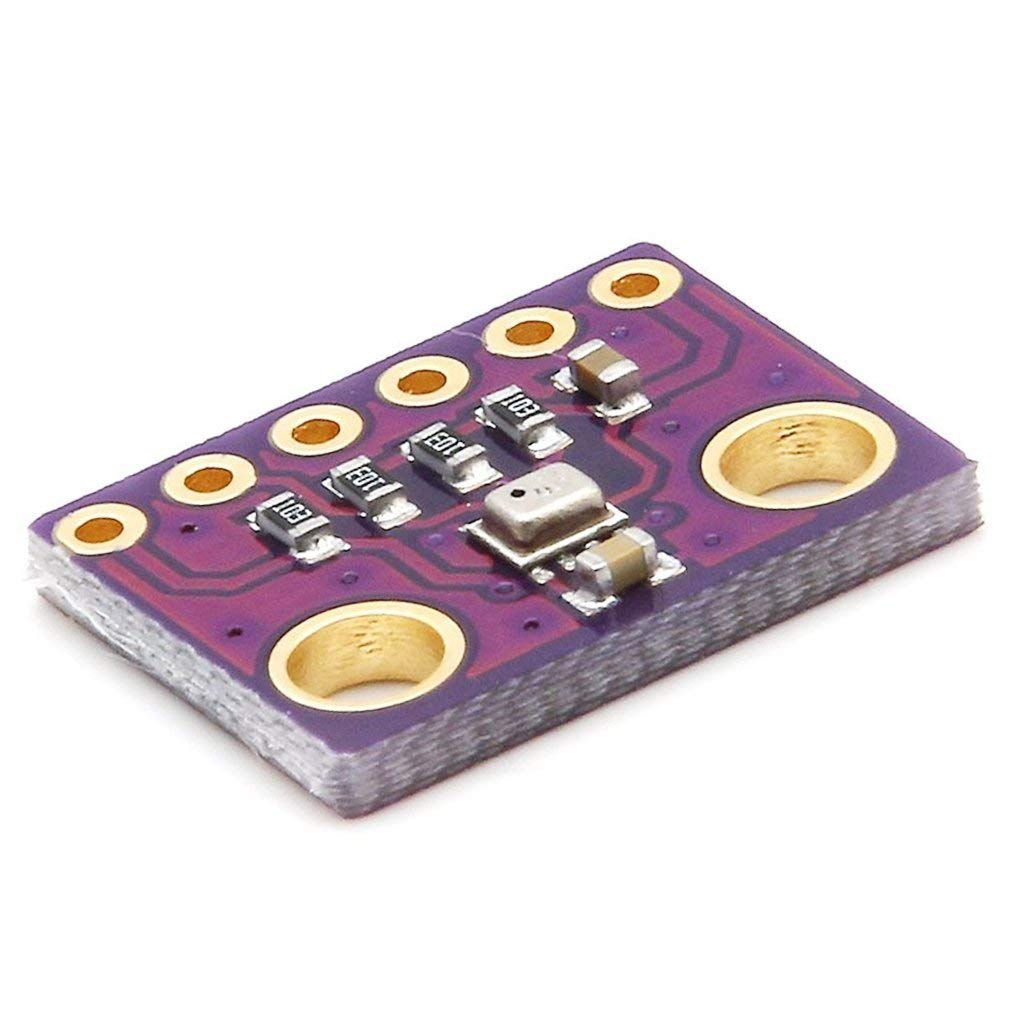
\includegraphics[width=0.4\textwidth]{Detector_description/bmp280.jpg}
  \caption{BMP280 sensor PCB example, it can be easily found online. Taken from \href{https://a.co/d/hhF7Vtp}{Amazon}.}
  \label{fig:bmp280}
\end{figure}

An absolute barometric pressure sensor \href{https://www.bosch-sensortec.com/products/environmental-sensors/pressure-sensors/bmp280/}{BMP280} can be included in the detector construction to make barometric measurements that can relate to muon counts. Temperature can also affect the SiPM and LYSO response, possibly making this data important while characterizing the detector. The Raspberry Pi Pico has a built-in temperature sensor, this however has been found to have some errors depending on the reference voltage, making its calibration necessary.

The Raspberry Pi Pico reads data from the BMP280 through the I2C protocol, the MicroPython driver can also be found in \href{https://github.com/dafvid/micropython-bmp280}{micropython-bmp280} by David Stenwall, who has made an amazing description on the use of this sensor in his repository.

\subsection{OLED screen}

\begin{figure}[H]
  \centering
  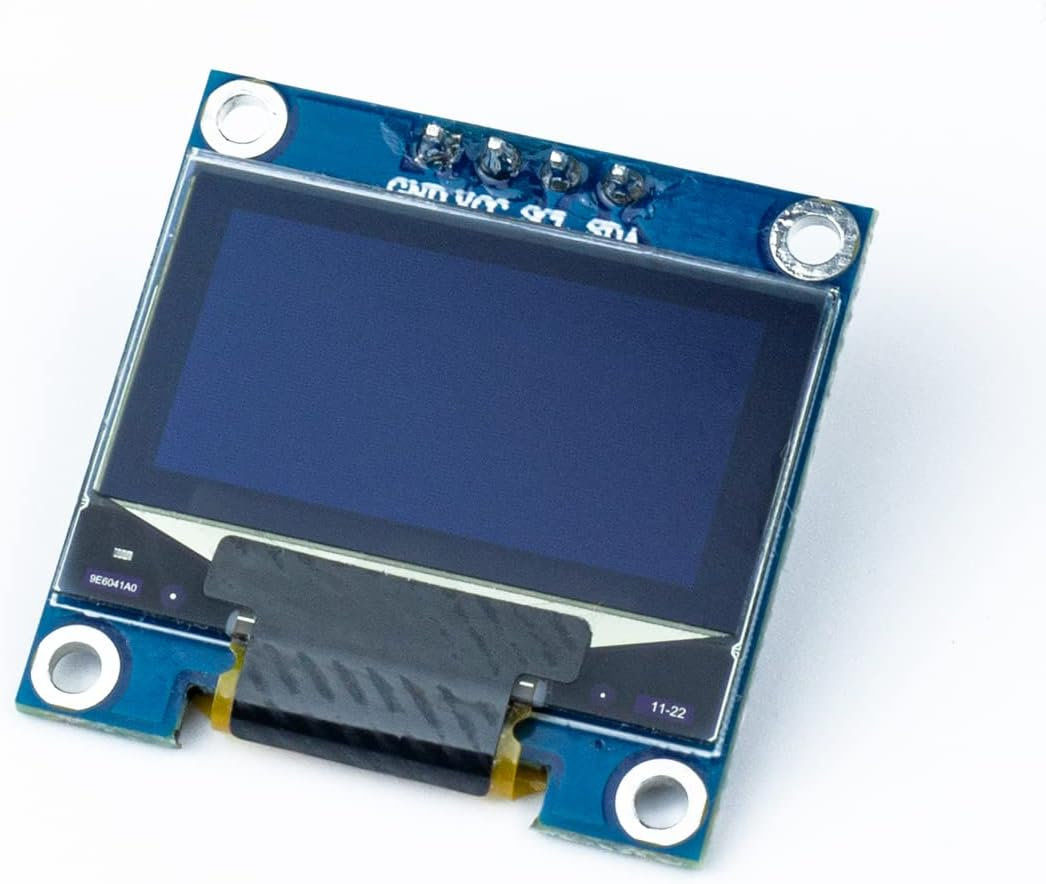
\includegraphics[width=0.4\textwidth]{Detector_description/ssd1306.jpg}
  \caption{SSD1306 OLED screen example, it can be easily found online. Taken from \href{https://a.co/d/cGnBDLF}{Amazon}}
  \label{fig:bssd1306}
\end{figure}

OLED screens are versatile and provide a fast way to read data directly from the detector, making it more user-friendly and easier to troubleshoot. An ssd1306 OLED screen can be connected to the detector, the driver is listed in the \href{https://github.com/micropython/micropython-lib/tree/master/micropython/drivers/display}{MicroPython documentation}.

The ``Log in'' screen of the detector shows a $128\times 64$ pixelart on bytearray form of the CosmicWatch logo, found under the ``Logos'' in \href{https://github.com/anvargasl/CosmicWatch-gamma-spectroscopy-RP}{CosmicWatch-gamma-spectroscopy-RP}.

\section{3D printed case}

In order to hold the crystal in place on the SiPM PCB, it was necessary to design a 3D printed case -see Fig. \ref{fig:3d_case_desing} for a schematic of the 3D design on Inventor. With this we made sure that the crystal would not move relative to the SiPM, preventing scratches and providing a more stable optical coupling with the photomultiplier.

\begin{figure}[H]
    \centering
    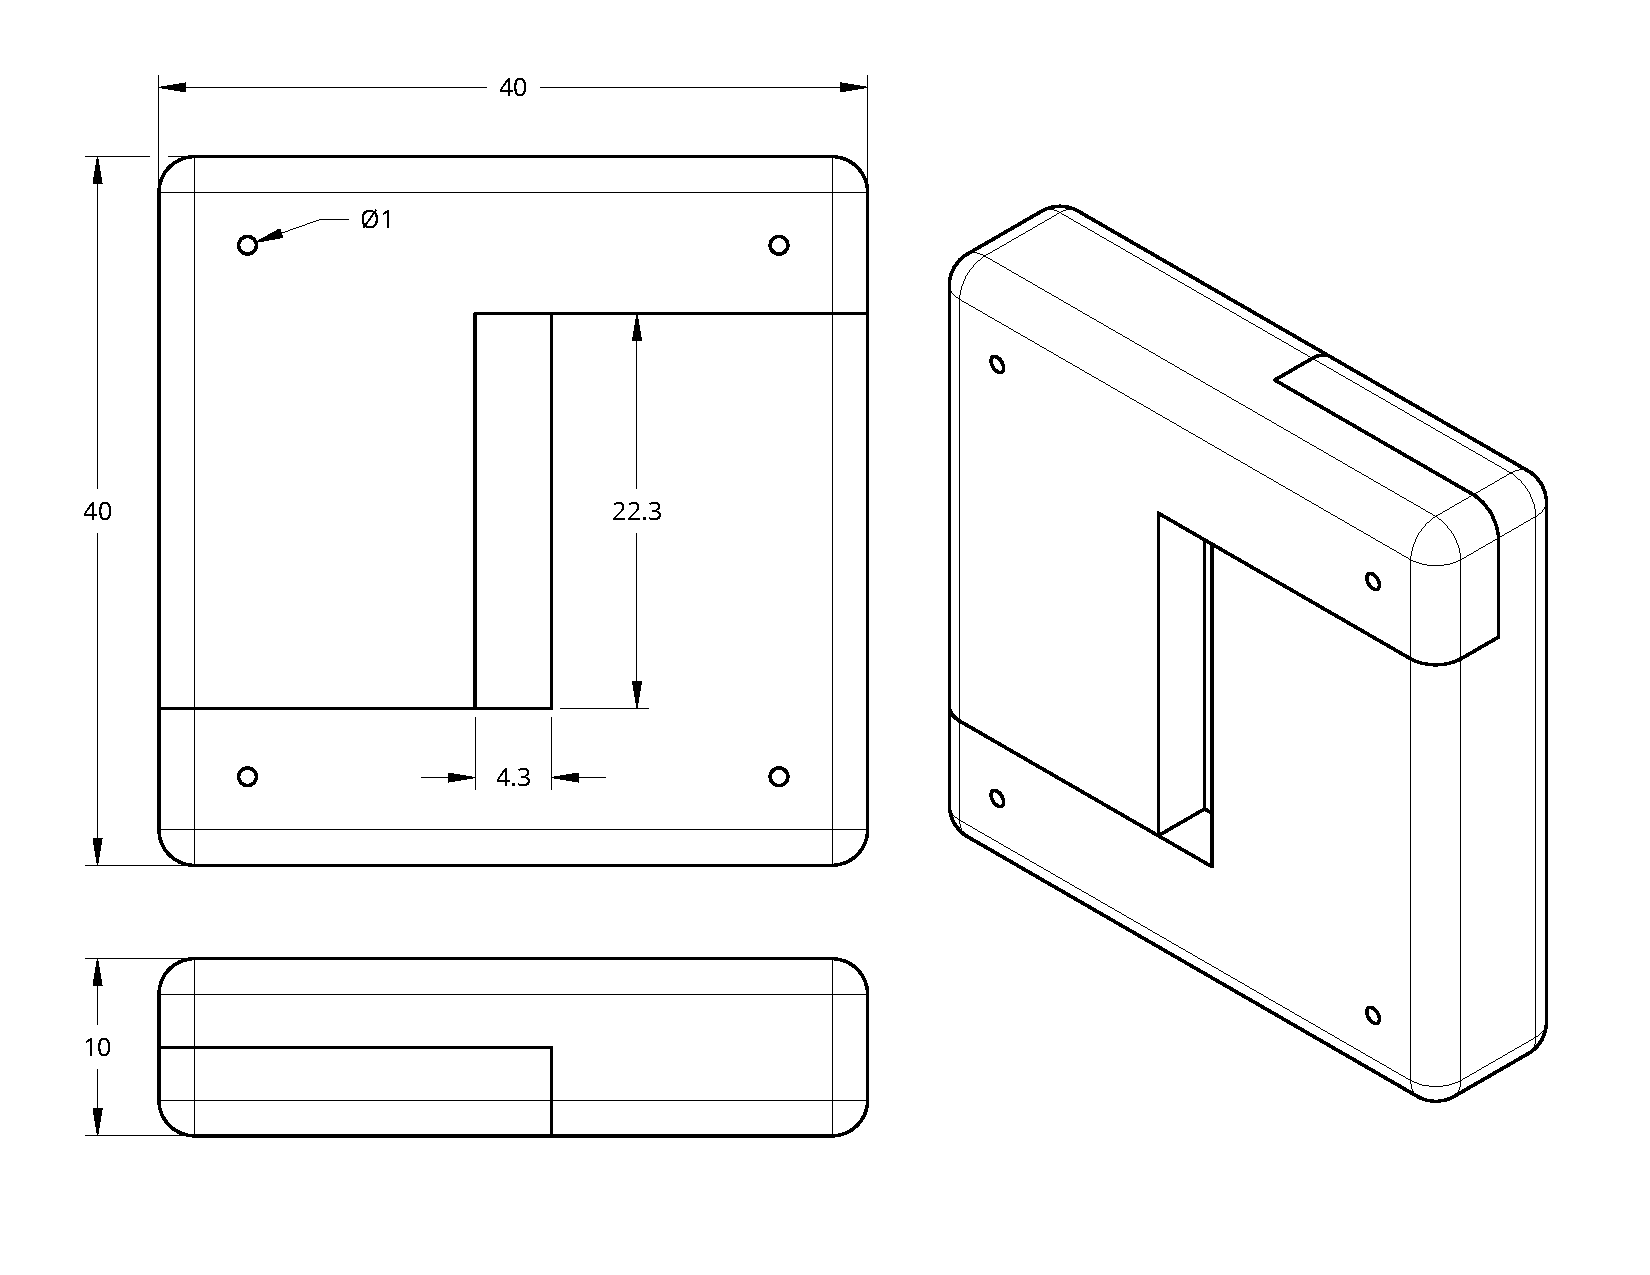
\includegraphics[width=\textwidth]{Detector_description/LYSO-holder-drawing.pdf}
    \caption{Case model for a $4\times4\times22$ \unit{mm\cubed} LYSO crystal, all dimensions are shown in \unit{\mm}. The \texttt{.stl} and \texttt{.ipt} files for 3D printing can be found on the repository \href{https://github.com/anvargasl/CosmicWatch-gamma-spectroscopy-PCB}{CosmicWatch-gamma-spectroscopy-PCB}.}
    \label{fig:3d_case_desing}
\end{figure}

The design keeps in mind that the crystal has to be wrapped in Teflon tape to increase reflectivity, which is why it comes in two pieces that come together around the crystal, lowering the risk of tears. Once the crystal is placed in the case it can be kept together using electrical tape.

Before using Teflon tape, the crystal was wrapped in tin foil, which made tears common (Fig. \ref{fig:tin_foil_tear}) and greatly impacted the quality of the spectra that could be obtained with the detector. 

\begin{figure}[H]
    \centering
    \begin{subfigure}[t]{0.45\textwidth}
      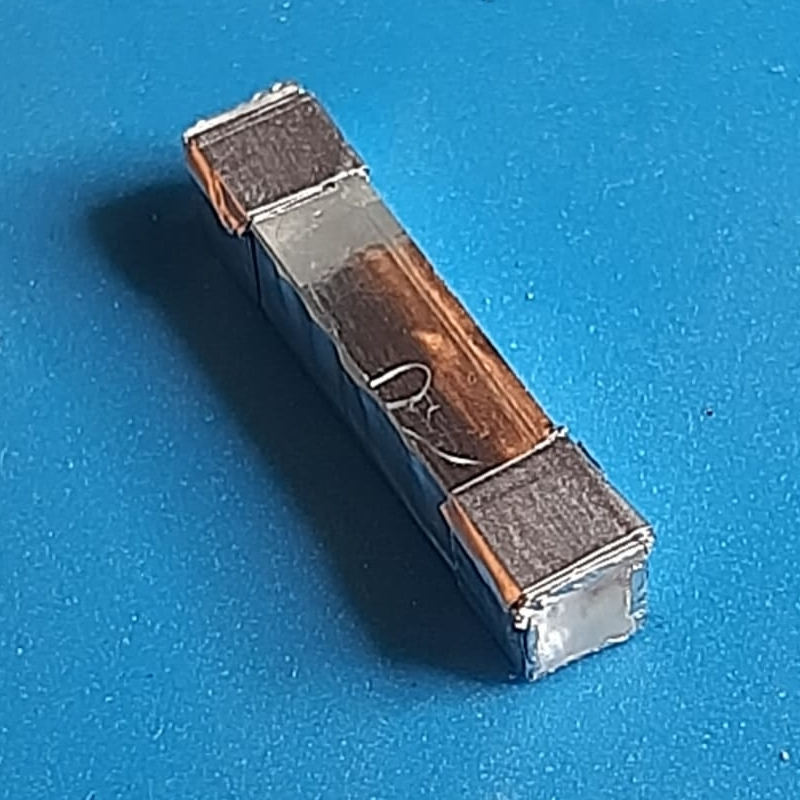
\includegraphics[width=\textwidth]{Detector_description/LYSO-wrapped.jpeg}
    \end{subfigure}
    \begin{subfigure}[t]{0.45\textwidth}
      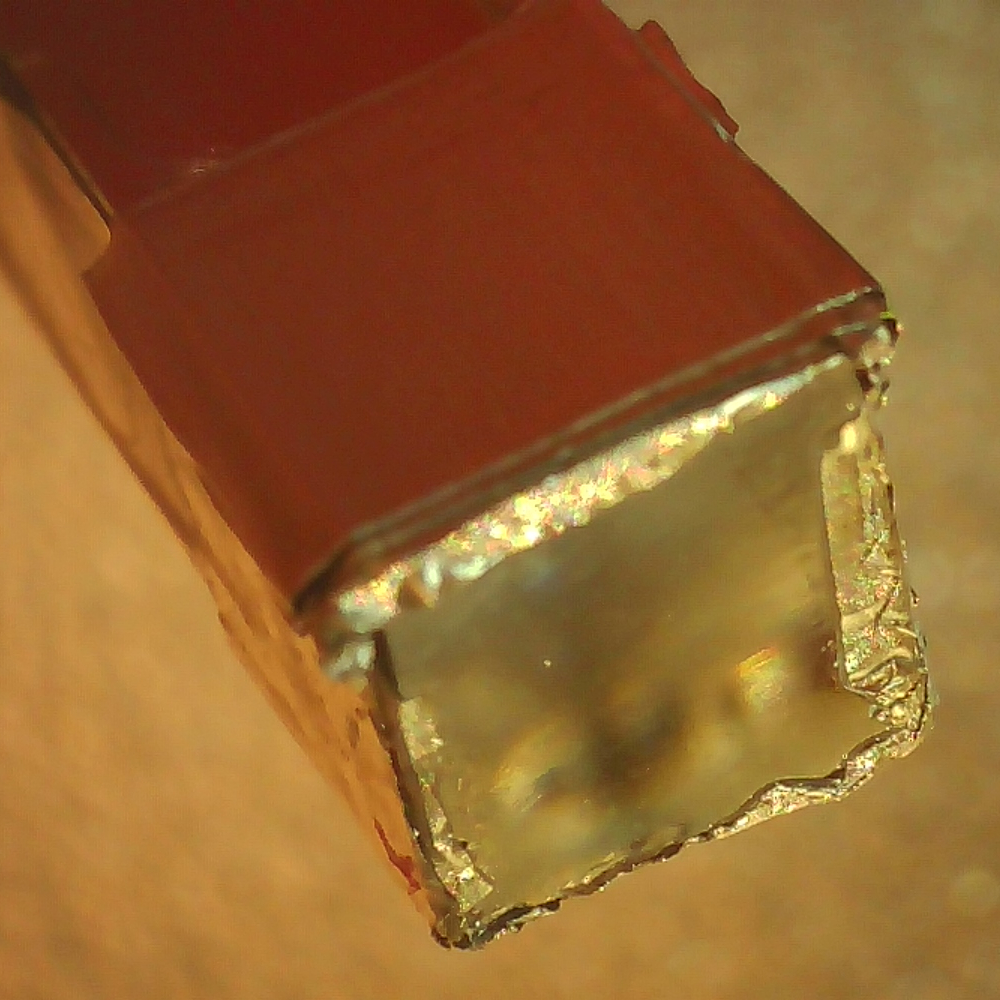
\includegraphics[width=\textwidth]{Detector_description/tin_foil_tear.jpg}
    \end{subfigure}
    \caption{\label{fig:tin_foil_tear}Tin foil tear.}
\end{figure}

Teflon tape seems to solve the tearing problem. However, to reduce the risk of tearing the Teflon, multiple iterations of the case were designed (Fig. \ref{fig:3d_previous_desings})

\begin{figure}[H]
    \centering
    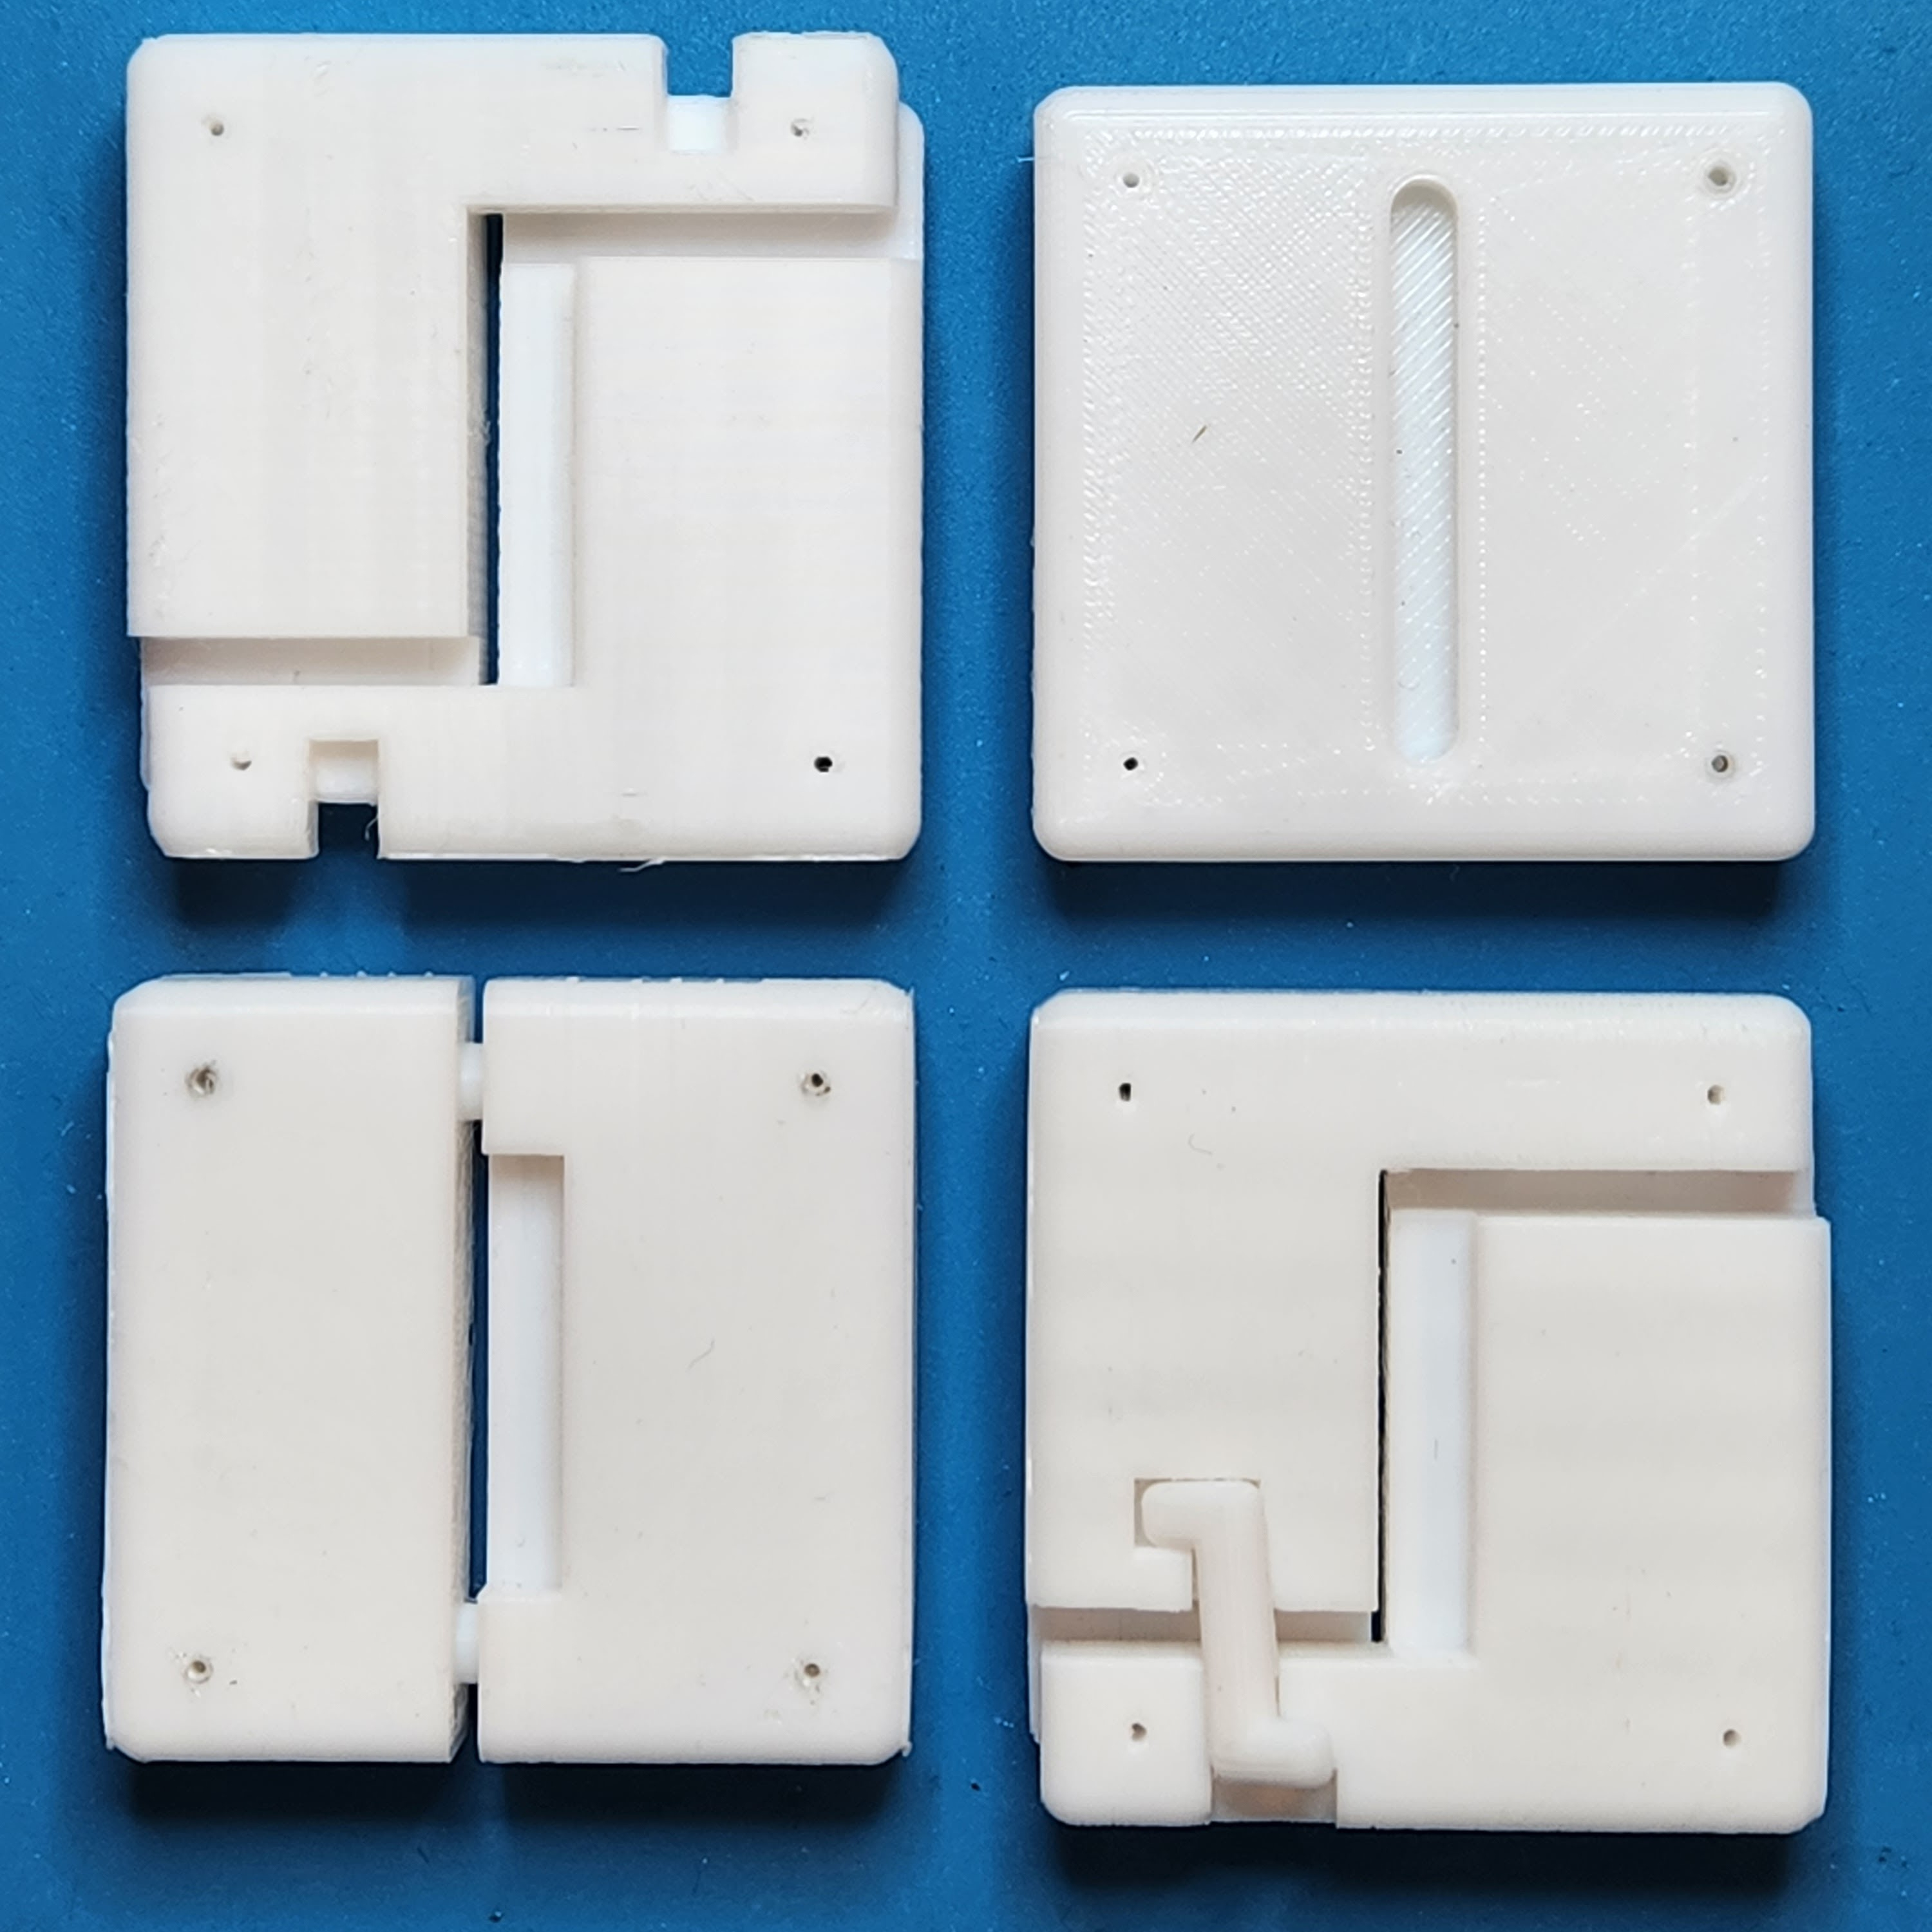
\includegraphics[width=0.6\textwidth]{Detector_description/Holder-designs.jpeg}
    \caption{3D printed cases tested to reduce the risk of Teflon tears.}
    \label{fig:3d_previous_desings}
\end{figure}
